\section{The manager object: \code{self.opx}}
\label{sec:manager}

Every kexp experiment gets an \code{OPXManager} as \code{self.opx} from
\code{Base.\_\_init\_\_}, through the lab factory
\code{make\_opx\_manager(self)}.\footnote{\file{k-exp/kexp/base/base.py}
lines 78--82; \file{k-exp/kexp/control/opx/opx\_config.py},
\code{make\_opx\_manager}.} It is constructed \emph{inert}: no \code{qm}
import, no network, nothing in a kernel. An experiment that never calls
\code{self.opx.use(...)} pays nothing, and \code{kexp} imports on analysis
machines without qm-qua installed. The manager is generic (no kexp imports);
the lab wires in the host/cluster, the channel-map builder and the config
builder through the factory.

\subsection{Lifecycle}

\begin{table}[htbp]
\centering
\small
\begin{tabular}{@{}lll@{}}
\toprule
experiment step & manager call & what happens \\
\midrule
\code{Base.\_\_init\_\_} & \code{make\_opx\_manager} & inert object; \code{host}, \code{cluster}, builders stored \\
\code{prepare()} & \code{self.opx.use(seq)} & resolve the sequence; build the channel map; check claims; refuse config-time xvars; resolve shapes; register DataVault containers; connect to the QMM \\
\code{finish\_prepare()} & \code{on\_finish\_prepare()} & shot tables $\to$ machine/config $\to$ trace $\to$ guards $\to$ provenance $\to$ \code{open\_qm} + \code{execute} (job parks on its first trigger) \\
\code{scan\_kernel()} & (none) & \code{handoff\_to\_quantum\_machines()} / \code{wait\_for\_quantum\_machines\_handback()} on the kernel \\
\code{analyze()} $\to$ \code{end()} & \code{finish()} & fetch streams, fill containers, sequence \code{finish} hook, halt the job; then \code{end\_wax} saves \\
process exit & \code{\_halt\_quietly} (atexit) & a crashed process never leaves a parked job \\
\bottomrule
\end{tabular}
\caption{The manager's lifecycle against the experiment.
\file{k-exp/kexp/control/opx/manager.py} (module docstring and the four
public methods); call sites in \file{k-exp/kexp/base/base.py}
(\code{finish\_prepare} line 119, \code{end} lines 330--336).}
\label{tab:lifecycle}
\end{table}

\subsubsection{\code{prepare()}: \code{self.opx.use(sequence)}}

\begin{lstlisting}[style=py]
# k-exp/kexp/experiments/qm/check_rabi_frequency_apd_opx.py, prepare()
self.opx.use(rabi_raman_pulse)
# self.opx.use(rabi_raman_pulse, simulate=True)   # waveform report, no run
self.finish_prepare(shuffle=False)
\end{lstlisting}

\code{use()} must be called before \code{finish\_prepare()} because it
registers data containers, and \code{data.init()} inside
\code{finish\_prepare\_wax} sizes every container by \code{xvardims}
(section~\ref{sec:data}). In order:\footnote{\file{manager.py},
\code{OPXManager.use}.}

\begin{enumerate}[nosep]
  \item \code{get\_sequence(sequence)}: an \code{OPXSequence} object or the
    registered name of one already imported. A bare function is refused --
    the decorator is what declares claims and measurements.
  \item The channel map is built now, and \code{cmap.spec(role)} is looked up
    for every claimed role, so an unknown role fails in \code{prepare()}.
  \item \code{check\_config\_time\_xvars}: any xvar already declared on a
    config-time parameter (section~\ref{sec:program:config}) is refused now,
    before a run id exists (the check runs again at \code{finish\_prepare}).
  \item The declared shapes are resolved against the live \code{ExptParams}
    (\code{seq.resolve\_measurements(params)} / \code{resolve\_host\_data}: an
    int $N$, a tuple such as $(N, m)$, a \code{Stream(shape, dtype)}, or a
    callable \code{lambda p: ...} returning one of those), and one
    \code{DataVault} container is registered per key: float64 for float
    streams and host data, int64 for int streams (timestamps); plus the two
    reserved int32 $(1,)$ containers \code{opx\_data\_valid} and
    \code{opx\_shot\_index}. A key colliding with a reserved name, an
    existing container or a DataVault attribute is refused.
  \item Last, \code{\_connect()}: the qm log gate is installed, \code{qm} is
    imported for the first time, and \code{QuantumMachinesManager(host,
    cluster\_name)} is created. An unreachable OPX raises \code{RuntimeError}
    here, in \code{prepare()}, so no run id is claimed for a run that cannot
    happen.
  \item Simulation flags are stored. \code{simulate=True} with
    \code{save\_data=True} prints a warning: a run id would be claimed for a
    run that never happens.
\end{enumerate}

\subsubsection{\code{finish\_prepare()}: \code{on\_finish\_prepare()}}

\code{Base.finish\_prepare} calls \code{finish\_prepare\_wax} first (repeats,
shuffle, derived params, container sizing, \code{INIT\_RUN} to liveOD) and
\emph{then} \code{self.opx.on\_finish\_prepare()}, ``after finish\_prepare\_wax
so the xvars are repeated and shuffled''.\footnote{\file{k-exp/kexp/base/base.py}
lines 101--119.} The manager then does, in this order:

\begin{enumerate}[nosep]
  \item \code{tables = build\_shot\_tables(expt)}: one deep copy of
    \code{ExptParams}, swept over every shot in execution order
    (section~\ref{sec:xvars:tables}).
  \item \code{self.\_map = kexp\_channel\_map(expt)}, then
    \code{check\_config\_time\_xvars} again with the map's
    \code{config\_time\_params}, then every config-time key is added to
    \code{tables.accessed} so the adjust guard covers it, then
    \code{config = build\_opx\_config(expt, tables)} $=$
    \code{build\_machine(expt, tables).generate\_config()}
    (section~\ref{sec:program:config}). The map -- and the \code{Machine} it
    carries for provenance -- is built \emph{with} the tables here
    (\code{\_call\_map\_builder(expt, tables)}: the lab's
    \code{kexp\_channel\_map} accepts them), so \code{opx\_machine} records
    the first executed shot's transition exactly as the config the job runs
    (\code{transition\_source = 'shot tables (first executed shot)'}); at
    \code{use()}, before the tables exist, it is compiled at the declared
    value.
  \item The declared shapes are resolved again and compared with those of
    \code{use()}: a parameter a shape depends on that changed in between is
    a \code{RuntimeError}.
  \item \code{OPXProgramBuilder(seq, map, tables, n\_shots).trace()}: the
    QUA program (section~\ref{sec:program}). The context's stream roles are
    kept for the volts conversion at the end.
  \item \code{check\_live\_adjust\_conflicts(expt, tables)}
    (section~\ref{sec:midloop:adjust}).
  \item \code{\_connect()} again (a no-op after \code{use()}; the provenance
    script below needs the connection, because \code{generate\_qua\_script}
    drops the config section without qm's capabilities).
  \item Provenance into \code{expt.\_extra\_file\_texts}
    (\code{\_write\_provenance}): \code{opx\_qua\_program}
    (\code{generate\_qua\_script(prog, config)}), \code{opx\_machine} (the
    component tree as JSON, when the map carries one) and
    \code{opx\_shot\_tables} (accessed columns, shapes, versions; the job id
    is appended after \code{execute}). \code{end\_wax} ships these in the
    \code{END\_RUN} payload and the liveOD \code{DataSaver} writes each as an
    HDF5 attribute (section~\ref{sec:data:file}).
  \item \code{simulate=True}: re-trace with \code{skip\_triggers=True} on
    tables sliced to the first \code{simulate\_shots} shots, run the QOP
    simulator, open the pulse viewer, and \code{SystemExit} before any ARTIQ
    hardware runs (unless driven from \code{OPXBench}).
  \item Otherwise \code{self.\_qm = qmm.open\_qm(config)}; \code{self.\_job =
    qm.execute(prog)}; \code{atexit.register(self.\_halt\_quietly)} once. The
    job runs its prologue and parks on the first \code{wait\_for\_trigger}.
\end{enumerate}

\subsubsection{Per shot: nothing on the host}

During the scan the manager does nothing. The ARTIQ kernel triggers the OPX
once per \code{scan\_kernel} and waits for the hand-back
(section~\ref{sec:handoff}); the OPX job advances its own shot counter.
Nothing ties the two counters together except ``exactly one trigger per
shot'' -- which is why the builder echoes the OPX counter into a stream
(section~\ref{sec:data:echo}).

\subsubsection{\code{end()}: \code{finish()}}

\code{Base.end} calls \code{self.opx.finish()} inside a \code{try} before
\code{end\_wax} serialises the DataVault; a failure is printed loudly and the
run is still saved (the OPX containers then keep their zero placeholders and
\code{opx\_data\_valid} is all zero, which reads correctly as ``no valid OPX
data'').\footnote{\file{k-exp/kexp/base/base.py} lines 325--336.}
\code{finish()} then:

\begin{enumerate}[nosep]
  \item \code{\_fetch\_streams}: for every declared key (including timestamp
    streams and the shot-index echo), wait until
    \code{count\_so\_far() >= min(n\_shots, expt.\_shot\_complete\_count)} or
    30\,s, then \code{fetch\_all()}. An aborted run simply has fewer shots.
  \item \code{fill\_containers}: NaN-filled targets, volts conversion only for
    streams produced by \code{ctx.measure}, reshape into the container grid,
    the 0/1 mask, the shot-index check (section~\ref{sec:data:fill}).
  \item \code{\_finished = True}, then the sequence's optional
    \code{finish(expt, data)} hook inside a \code{try}/\code{finally} whose
    \code{finally} is \code{\_halt\_quietly} (\code{job.halt()} and
    \code{qm.close()}). Because \code{\_finished} is set only after a
    successful fetch and fill, a transient timeout leaves the job running
    and a second \code{finish()} retries from scratch; a hook error is raised
    to the caller with the raw containers already filled.
\end{enumerate}

\subsection{Sequence diagram}

\begin{figure}[htbp]
\centering
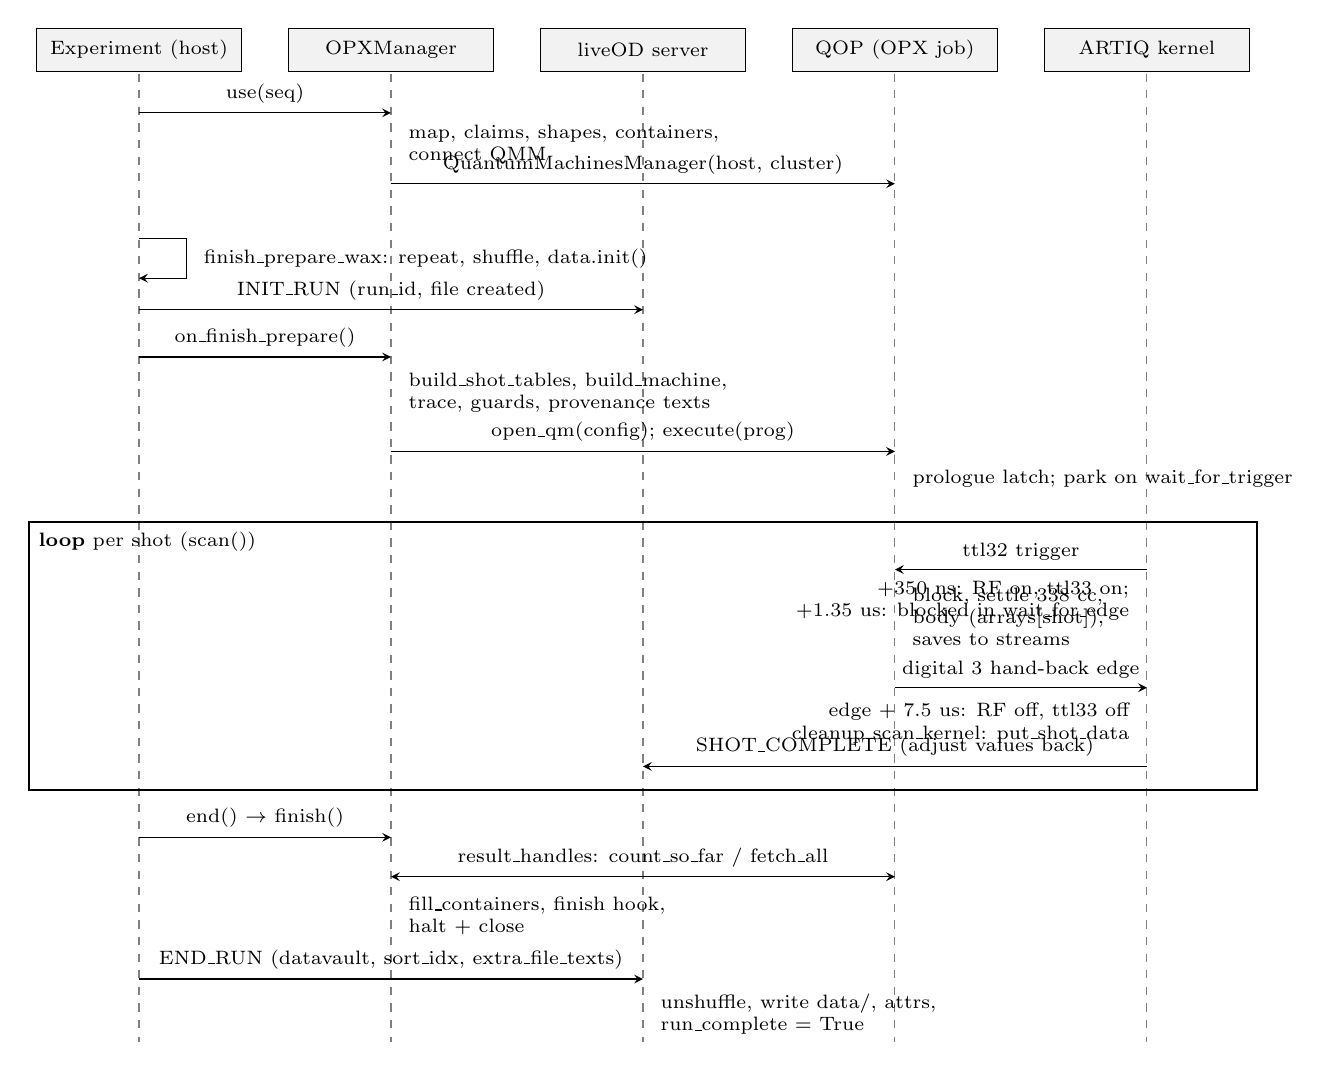
\begin{tikzpicture}[>=stealth, font=\scriptsize, x=1cm, y=1cm]
  % lifelines
  \foreach \x/\name in {0/Experiment (host), 3.2/OPXManager, 6.4/liveOD server, 9.6/QOP (OPX job), 12.8/ARTIQ kernel} {
    \node[draw, fill=gray!10, minimum width=2.6cm, minimum height=0.55cm] at (\x,0) {\name};
    \draw[dashed, gray] (\x,-0.3) -- (\x,-12.6);
  }
  % prepare
  \draw[->] (0,-0.8) -- (3.2,-0.8) node[midway, above] {use(seq)};
  \node[anchor=west, align=left] at (3.3,-1.2) {map, claims, shapes, containers,\\connect QMM};
  \draw[->] (3.2,-1.7) -- (9.6,-1.7) node[midway, above] {QuantumMachinesManager(host, cluster)};
  % finish_prepare
  \draw[->] (0,-2.4) -- (0.6,-2.4) -- (0.6,-2.9) -- (0,-2.9);
  \node[anchor=west] at (0.7,-2.65) {finish\_prepare\_wax: repeat, shuffle, data.init()};
  \draw[->] (0,-3.3) -- (6.4,-3.3) node[midway, above] {INIT\_RUN (run\_id, file created)};
  \draw[->] (0,-3.9) -- (3.2,-3.9) node[midway, above] {on\_finish\_prepare()};
  \node[anchor=west, align=left] at (3.3,-4.35) {build\_shot\_tables, build\_machine,\\trace, guards, provenance texts};
  \draw[->] (3.2,-5.1) -- (9.6,-5.1) node[midway, above] {open\_qm(config); execute(prog)};
  \node[anchor=west] at (9.7,-5.45) {prologue latch; park on wait\_for\_trigger};
  % run loop
  \draw[thick] (-1.4,-6.0) rectangle (14.2,-9.4);
  \node[anchor=north west] at (-1.4,-6.0) {\textbf{loop} per shot (scan())};
  \draw[->] (12.8,-6.6) -- (9.6,-6.6) node[midway, above] {ttl32 trigger};
  \node[anchor=east, align=right] at (12.7,-7.0) {+350 ns: RF on, ttl33 on;\\+1.35 us: blocked in wait\_for\_edge};
  \node[anchor=west, align=left] at (9.7,-7.2) {block, settle 338 cc,\\body (arrays[shot]),\\saves to streams};
  \draw[->] (9.6,-8.1) -- (12.8,-8.1) node[midway, above] {digital 3 hand-back edge};
  \node[anchor=east, align=right] at (12.7,-8.55) {edge + 7.5 us: RF off, ttl33 off\\cleanup\_scan\_kernel: put\_shot\_data};
  \draw[->] (12.8,-9.1) -- (6.4,-9.1) node[midway, above] {SHOT\_COMPLETE (adjust values back)};
  % end
  \draw[->] (0,-10.0) -- (3.2,-10.0) node[midway, above] {end() $\to$ finish()};
  \draw[<->] (3.2,-10.5) -- (9.6,-10.5) node[midway, above] {result\_handles: count\_so\_far / fetch\_all};
  \node[anchor=west, align=left] at (3.3,-11.0) {fill\_containers, finish hook,\\halt + close};
  \draw[->] (0,-11.8) -- (6.4,-11.8) node[midway, above] {END\_RUN (datavault, sort\_idx, extra\_file\_texts)};
  \node[anchor=west, align=left] at (6.5,-12.25) {unshuffle, write data/, attrs,\\run\_complete = True};
\end{tikzpicture}
\caption{Who talks to whom, in order. The host never touches the OPX during
the scan; the per-shot coupling is purely the two TTL wires between the
kernel and the job. Sources: \file{manager.py} (\code{use},
\code{on\_finish\_prepare}, \code{finish}); \file{wax/waxx-src/waxx/base/expt.py}
(\code{finish\_prepare\_wax}, \code{end\_wax}, \code{\_notify\_shot\_complete});
\file{k-exp/kexp/base/control.py} (the two handshake kernels).}
\label{fig:sequence}
\end{figure}

\subsection{Interactive use: \code{OPXBench}}

\code{OPXBench} stands in for a prepared experiment in a notebook: real
\code{ExptParams}, the real \code{dds\_frame} defaults, an \code{xvar}
interface, no ARTIQ, no liveOD, no run id.\footnote{\file{k-exp/kexp/control/opx/bench.py}.}
\code{bench.simulate(seq, shots=2)} runs \code{use(simulate=True)} +
\code{on\_finish\_prepare()} with \code{\_exit\_after\_simulate = False}, returns
the simulator job and opens the pulse viewer. Its \code{xvar} runs values in
the order given (no shuffle, no repeats), so shot $k$ of the simulation is
\code{values[k]}. It constructs \code{self.raman} as a real
\code{RamanBeamPair} exactly as \file{kexp/base/devices.py} does, so the
Raman transition split (\code{raman\_transition\_to\_ifs}) is the lab's; this
is how the feedback port was compiled and timed on the QOP simulator. Its
\code{compute\_new\_derived} is a no-op, so a sequence that reads an
experiment-local derived parameter raises \code{AttributeError} from
\code{ctx.p} on the bench.
